\documentclass[xcolor=dvipsnames]{beamer}

\usetheme{Darmstadt}
\usefonttheme[onlylarge]{structurebold}
\setbeamerfont*{frametitle}{size=\normalsize,series=\bfseries}
\setbeamertemplate{navigation symbols}{}

\usepackage[english]{babel}
\usepackage[cp1250]{inputenc}
\usepackage{times}
\usepackage[T1]{fontenc}


\usepackage{graphicx,amsmath} % Add all your packages here
\usepackage{amsfonts}
%\usepackage{listings}


\usepackage{url}

\usepackage{tikz}
\usetikzlibrary{arrows}
\tikzstyle{block}=[draw opacity=0.7,line width=1.4cm]


% correct bad hyphenation here
\hyphenation{op-tical net-works semi-conduc-tor IEEEtran}


\title{Fuzzy ILP classifier for Weka}

\author[D�dek]
{Jan D�dek}

\institute[MFF UK]
{
Department of Software Engineering, Faculty of Mathematics and Physics, Charles University in Prague, Czech Republic
}

\date[SAIAW WI 2009]
{Tools Demo Session,\\WDS, 2nd June 2010, MFF UK, Troja, Prague 8\\
\bigskip \url{http://www.ksi.mff.cuni.cz/~dedek/fuzzyILP/}}



\begin{document}

\begin{frame}
  \titlepage
\end{frame}

%\begin{frame}{Outline}
%  \tableofcontents
%\end{frame}



\section{Fuzzy ILP}

\subsection{Introd. example, theory, architecture and an experiment}
\frame{\tableofcontents[currentsubsection]}

\begin{frame}[fragile]{ILP Example}
\begin{block}{Types of ground variables}
{\footnotesize\begin{verbatim}
animal(dog). animal(dolphin) ... animal(penguin).
class(mammal). class(fish). class(reptile). class(bird).
covering(hair). covering(none). covering(scales).
habitat(land). habitat(water). habitat(air).
\end{verbatim}}
\end{block}
\begin{block}{Background knowledge}
{\footnotesize\begin{verbatim}
has_covering(dog, hair). has_covering(crocodile, scales).
has_legs(dog,4). ... has_legs(penguin, 2). etc.
has_milk(dog). ... has_milk(platypus). etc.
homeothermic(dog). ... homeothermic(penguin). etc.
habitat(dog, land). ... habitat(penguin, water). etc.
has_eggs(platypus). ... has_eggs(eagle). etc.
has_gills(trout). ... has_gills(eel). etc.
\end{verbatim}}
\end{block}
\end{frame}

\begin{frame}[fragile]{ILP Example}
\begin{columns}
\column{.5\textwidth}
\begin{block}{Positive examples}
{\footnotesize\begin{verbatim}
class(lizard, reptile).
class(trout, fish).
class(bat, mammal).
\end{verbatim}}
\end{block}
\column{.5\textwidth}
\begin{block}{Negative examples}
{\footnotesize\begin{verbatim}
class(trout, mammal).
class(herring, mammal).
class(platypus, reptile).
\end{verbatim}}
\end{block}
\end{columns}
\bigskip
\begin{block}{Induced rules}
{\footnotesize\begin{verbatim}
class(A,reptile) :- has_covering(A,scales),
                    has_legs(A,4).
class(A,mammal) :- homeothermic(A), has_milk(A).
class(A,fish) :- has_legs(A,0), has_eggs(A).
class(A,reptile) :- has_covering(A,scales),
                    habitat(A,land).
class(A,bird) :- has_covering(A,feathers).
\end{verbatim}}
\end{block}
\end{frame}




\begin{frame}{Classical ILP and Fuzzy ILP principles}
\begin{itemize}
	\item Learning examples $E=P\cup N$ (Positive and Negative)
	\item Background knowledge $B$
	\item ILP task -- to find hypothesis $H$ such that:
\end{itemize}
$$
(\forall e\in P)(B\cup H\models e) \ \ \&\  \ (\forall n\in N)(B\cup H\not\models n).
$$
\vspace{0.5cm}
\begin{itemize}
	\item Fuzzy learning examples ${\mathcal E}:E\longrightarrow [0,1]$
	\item Fuzzy background knowledge ${\mathcal B}:B\longrightarrow [0,1]$
	\item Fuzzy ILP task -- to find hyp. ${\mathcal H}:H\longrightarrow [0,1]$ such that:
\end{itemize}
$$
(\forall e_1,e_2\in E)(\forall {\mathcal M})({\mathcal M}\models_f {\mathcal B}\cup {\mathcal H}) \ :\ 
{\mathcal E}(e_1)>{\mathcal E}(e_2)\Rightarrow \left\|e_1\right\|_{{\mathcal M}}\ge \left\|e_2\right\|_{{\mathcal M}}
$$
\end{frame}

\begin{frame}{Generalized Annotated Programs}
\begin{itemize}
	\item Fuzzy ILP is equivalent to Induction of Generalized Annotated Programs\footnote{See in S. Krajci, R. Lencses and P. Vojtas: ``A comparison of fuzzy and annotated logic programming'', Fuzzy Sets and Systems, vol.144, pp.173�192, 2004.}
	\item For implementation we use GAP or strictly speaking: \emph{Definite Logic Programs with monotonicity axioms} (also equivalent)
	\item Basic paradigm: deal with \alert{values} as with \alert{degrees}.
		\begin{itemize}
			\item We don't have to normalize values, they order is enough.			
		\end{itemize}
	\medskip
	\item For example with monotonicity axioms we can use rule:
\centerline{\texttt{serious(A, 4)} $\leftarrow$ \texttt{fatalities(A, 10).}}
and from the fact \texttt{fatalities(id\_123, 1000)} deduce
\centerline{\texttt{serious\_alt(id\_123, 4).}}
\end{itemize}
\end{frame}


\begin{frame}{Schema of the whole system}
\begin{columns}
\column{.45\textwidth}
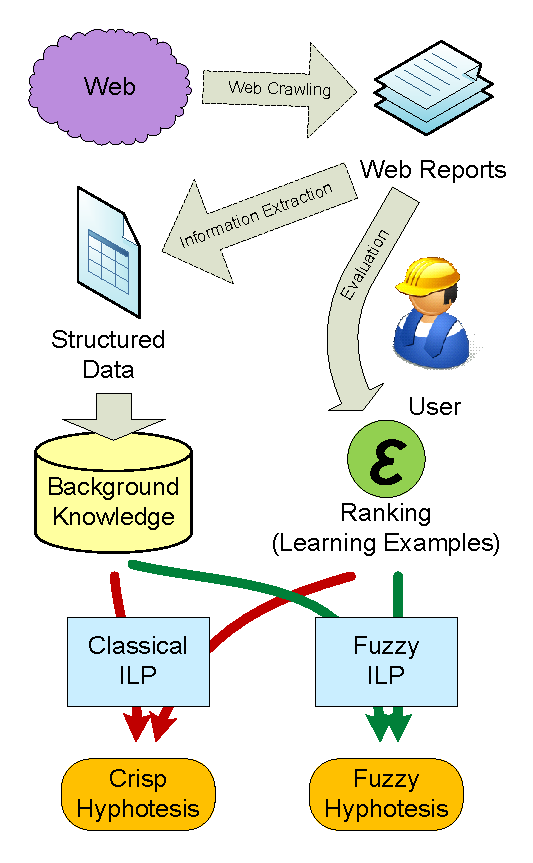
\includegraphics[height=0.9\vsize]{img/schema}
\column{.55\textwidth}
\begin{enumerate}
	\item Web Crawling
	\item Information Extraction and User Evaluation
	\item Logic representation
		\begin{itemize}
			\item Construction of \alert{background knowledge}
			\item Construction of \alert{learning examples}
		\end{itemize}
	\item ILP Learning
		\begin{itemize}
			\item Crisp
			\item Fuzzy
		\end{itemize}		
	\bigskip
	\item Comparison of results
\end{enumerate}
\end{columns}
\end{frame}


\begin{frame}{Accident attributes}
\begin{columns}
\column{.6\textwidth}
\includegraphics[height=0.75\vsize]{img/attributes_description}
\column{.4\textwidth}
\begin{itemize}
	\item Information that could be extracted.
	\item Missing values.
	\item Almost all attributes are \alert{numeric}.
		\begin{itemize}
			\item So \alert{monotonic}
			\item This will be used for ``fuzzyfication''
		\end{itemize}
	\item Artificial target attribute \alert{seriousness ranking}.
\end{itemize}
\end{columns}
\end{frame}


\begin{frame}{Histogram of the seriousness ranking attribute}
\includegraphics[width=0.9\hsize]{img/ranking_histogram}
\begin{itemize}
	\item 14 different values, range 0.5 -- 8
	\item Divided into four approximately \alert{equipotent groups}.
\end{itemize}
\end{frame}





\subsection{Fuzzy ILP Implementation}
\frame{\tableofcontents[currentsubsection]}

\begin{frame}{Essential difference between learning examples}
\begin{columns}
\column{.6\textwidth}
\setbeamercolor{block title}{bg=BrickRed}
\begin{block}{Crisp learning examples}
\centerline{\includegraphics[width=\hsize]{img/examples_nonmonot}}
\end{block}
\bigskip
\setbeamercolor{block title}{bg=OliveGreen}
\begin{block}{Monotonized learning examples}
\centerline{
\includegraphics[width=\hsize]{img/examples_monot}}
\end{block}
\column{.4\textwidth}
For one evidence (occurrence):
	\bigskip
\begin{itemize}
	\item Crisp:\\
	Always \alert{one} positive and \alert{three} negative learning examples
	\bigskip
	\item Monotonized:\\
	\alert{Up to the observed degree} positive,\\the rest negative.
\end{itemize}
\end{columns}
\end{frame}


\begin{frame}{Monotonization of attributes}
\definecolor{MyBrown}{rgb}{0.5,0.5,0}
\setbeamercolor{block title}{bg=MyBrown}
\begin{block}{damage\_atl $\leftarrow$ damage}
\centerline{\includegraphics[width=0.73\hsize]{img/attribute_monotonisation}}
\end{block}
\bigskip
\begin{itemize}
	\item We infer all lower values as sufficient.
	\item Treatment of unknown values.
	\item Negation as failure.
\end{itemize}
\end{frame}

\subsection{Evaluation}
\frame{\tableofcontents[currentsubsection]}


\begin{frame}[plain]%{Crisp \& monotonized hypothesis}
\begin{columns}
\column{.67\textwidth}
\centerline{
\includegraphics[height=1.1\vsize,width=\hsize]{img/rules}}
\column{.33\textwidth}
\begin{itemize}
	\item Crisp hypothesis
\vspace{3cm}
	\item Monotonized hypothesis	
	\begin{itemize}
		\item Monotonicity axioms
		\item Monotonized learning examples
	\end{itemize}
\end{itemize}
\vspace{2cm}
\end{columns}
\end{frame}


\begin{frame}{Evaluation and Comparison of Results -- graph}
\centerline{\includegraphics[width=1.16\hsize]{img/2x10cross}}
\end{frame}

\begin{frame}[plain]%{Evaluation and Comparison of Results -- table}
\hspace*{-0.8cm}
\scriptsize
{\centering \begin{tabular}{lr@{\hspace{0cm}}c@{\hspace{0cm}}rr@{\hspace{0cm}}c@{\hspace{0cm}}r@{\hspace{0.05cm}}cr@{\hspace{0cm}}c@{\hspace{0cm}}r@{\hspace{0.05cm}}cr@{\hspace{0cm}}c@{\hspace{0cm}}r@{\hspace{0.05cm}}cr@{\hspace{0cm}}c@{\hspace{0cm}}r@{\hspace{0.05cm}}cr@{\hspace{0cm}}c@{\hspace{0cm}}r@{\hspace{0.05cm}}cr@{\hspace{0cm}}c@{\hspace{0cm}}r@{\hspace{0.05cm}}c}
\\
\hline
& \multicolumn{3}{c}{Fuzzy}& \multicolumn{4}{c}{Crisp} & \multicolumn{4}{c}{MultPerc} & \multicolumn{4}{c}{SMO} & \multicolumn{4}{c}{J48} & \multicolumn{4}{c}{JRip} & \multicolumn{4}{c}{LBoost} \\
\hline
Corr	& 0.61 & $\pm$ & .19 & .22 & $\pm$ & .17 & $\bullet$ & .41 & $\pm$ & .19 & $\bullet$ & .36 & $\pm$ & .24 & $\bullet$ & .41 & $\pm$ & .22 & $\bullet$ & .44 & $\pm$ & .17 & $\bullet$ & .59 & $\pm$ & .26 &        \\
Incor	& .39 & $\pm$ & .19 & .27 & $\pm$ & .24 &         	& .59 & $\pm$ & .19 & $\circ$ 	& .64 & $\pm$ & .24 & $\circ$ 	& .59 & $\pm$ & .22 & $\circ$ 	& .56 & $\pm$ & .17 & $\circ$ 	& .41 & $\pm$ & .26 &        \\
Uncl	& .00	& $\pm$ & .00	& .51 & $\pm$ & .29 & $\circ$ 	& .00 & $\pm$ & .00 &         	& .00 & $\pm$ & .00 &         	& .00 & $\pm$ & .00 &         	& .00 & $\pm$ & .00 &         	& .00 & $\pm$ & .00 &        \\
Prec	& .56 & $\pm$ & .24 & .53 & $\pm$ & .37 &         	& .35 & $\pm$ & .20 & $\bullet$ & .33 & $\pm$ & .26 &         	& .39 & $\pm$ & .22 &         	& .34 & $\pm$ & .21 & $\bullet$ & .56 & $\pm$ & .28 &        \\
Rec		& .61 & $\pm$ & .19 & .49 & $\pm$ & .32 &         	& .41 & $\pm$ & .19 & $\bullet$ & .36 & $\pm$ & .24 & $\bullet$ & .41 & $\pm$ & .22 & $\bullet$ & .44 & $\pm$ & .17 & $\bullet$ & .59 & $\pm$ & .26 &        \\
F			& .56 & $\pm$ & .20 & .49 & $\pm$ & .33 &         	& .36 & $\pm$ & .19 & $\bullet$ & .32 & $\pm$ & .24 & $\bullet$ & .39 & $\pm$ & .21 &         	& .36 & $\pm$ & .19 & $\bullet$ & .56 & $\pm$ & .27 &        \\
\hline
\multicolumn{21}{c}{$\circ$, $\bullet$ statistically significant improvement or degradation}\\
\end{tabular} \scriptsize \par}
\scriptsize
\smallskip

\hspace*{-1.1cm}
{\centering
\begin{tabular}{p{2cm}@{}p{10.5cm}}\\
Fuzzy \dotfill{}& czsem.ILP.FuzzyILPClassifier '' \\
Crisp \dotfill{} & czsem.ILP.CrispILPClassifier '' \\
MultPerc \dotfill{} & functions.MultilayerPerceptron '-L 0.3 -M 0.2 -N 500 -V 0 -S 0 -E 20 -H a' \\
SMO \dotfill{} & functions.SMO '-C 1.0 -L 0.0010 -P 1.0E-12 -N 0 -V -1 -W 1 -K \textbackslash"functions.supportVector.PolyKernel -C 250007 -E 1.0\textbackslash"' \\
J48 \dotfill{} & trees.J48 '-C 0.25 -M 2' \\
JRip \dotfill{} & rules.JRip '-F 3 -N 2.0 -O 2 -S 1' \\
LBoost \dotfill{} & meta.LogitBoost '-P 100 -F 0 -R 1 -L -1.7976931348623157E308 -H 0.1 -S 1 -I 10 -W trees.DecisionStump' \\
\\
Corr \dotfill{} & Percent correct\\
Inor \dotfill{} & Percent incorrect\\
Uncl \dotfill{} & Percent unclassified\\
Prec \dotfill{} & Weighted avg IR precision\\
Rec \dotfill{} 	& Weighted avg IR recall\\
F \dotfill{} 		& Weighted avg F measure\\
\end{tabular}
}
%\caption{Evaluation of the methods in 2 times 10-fold cross validation.}
\end{frame}

%\begin{frame}{Evaluation and Comparison of Results}
%\centerline{\includegraphics[width=0.75\hsize]{img/Evaluation}}
%\bigskip
%\begin{itemize}
%	\item Rules evaluated on both testing sets.
%		\begin{itemize}
%			\item By use of conversion predicates (next slide)
%		\end{itemize}
%	\item Monotonized rules \alert{better in both cases}.
%	\item Even better than \alert{other classifiers} (Znalosti 2010).
%\end{itemize}
%\end{frame}



\begin{frame}{Conversion of Results}
\setbeamercolor{block title}{bg=BrickRed}
\begin{block}{crisp $\leftarrow$ monotone (select max)}
\centerline{\includegraphics[width=.8\hsize]{img/monot2nomon}}
\end{block}
\bigskip
\setbeamercolor{block title}{bg=OliveGreen}
\begin{block}{monotone $\leftarrow$ crisp}
\centerline{\includegraphics[width=.8\hsize]{img/nomon2monot}}
\end{block}
\end{frame}

%\section{Conclusion}
%\begin{frame}{Summary}
% \begin{itemize}
%  \item Proposed a system for extraction of semantic information 
%  \item Based on linguistic tools for automatic text annotation
%  \item Extraction rules adopted from \alert{Netgraph} application.
%  \item ILP used for learning rules.
%\bigskip
%  \item Our future research will concentrate on:  
%		\begin{itemize}
%			\item \alert{Learning} of extraction rules.
%			\item Extension of the method with WordNet technology.
%			\item Adaptation of this method on \alert{other languages}.
%			\item \alert{Evaluation} of the method.
%		\end{itemize}
% \end{itemize}
%\end{frame}

% no key words


\end{document}



%%% Local Variables: 
%%% mode: latex
%%% TeX-master: t
%%% End: 
